\documentclass[tikz,border=2pt]{standalone}
\usepackage{amsmath}
\usepackage{pgfplots}
\pgfplotsset{compat=1.18}
\usetikzlibrary{arrows.meta}
\begin{document}
% Left: K={-x2<=0, -x1+x2<=0} is the intersection of two halfspaces through 0 with row normals (0,-1),(-1,1);
% the generators (1,0),(1,1) lie on the walls. Right: V={x1+x2>=2, x>=0} = K+Q with K the nonnegative quadrant
% and Q the segment from (2,0) to (0,2); (3,1)=(1.5,0.5)+(1.5,0.5).
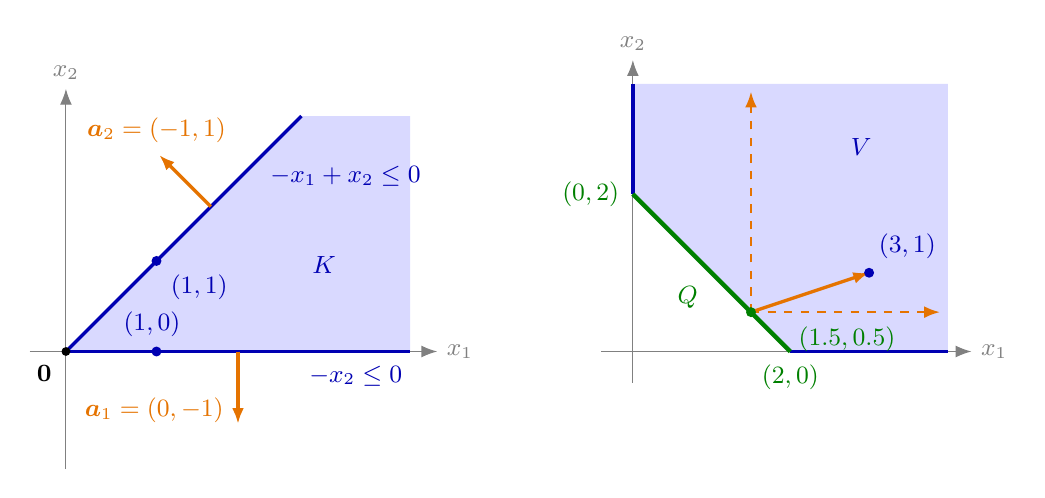
\begin{tikzpicture}[font=\small, >={Latex[length=2mm]}]
  % ---------- left panel: walls through the origin
  \begin{scope}[x=1.15cm, y=1.15cm]
    \fill[blue!15] (0,0) -- (3.8,0) -- (3.8,2.6) -- (2.6,2.6) -- cycle;
    \draw[gray, ->] (-0.4,0) -- (4.1,0) node[anchor=west] {$x_1$};
    \draw[gray, ->] (0,-1.3) -- (0,2.9) node[anchor=south] {$x_2$};
    \draw[blue!70!black, very thick] (0,0) -- (3.8,0);
    \draw[blue!70!black, very thick] (0,0) -- (2.6,2.6);
    \node[blue!70!black, anchor=north west] at (2.15,2.15) {$-x_1+x_2\leq0$};
    \node[blue!70!black, anchor=north] at (3.2,-0.05) {$-x_2\leq0$};
    \draw[orange!90!black, very thick, ->] (1.9,0) -- (1.9,-0.8);
    \node[orange!90!black, anchor=east] at (1.85,-0.65) {$\boldsymbol{a}_1=(0,-1)$};
    \draw[orange!90!black, very thick, ->] (1.6,1.6) -- (1.03,2.17);
    \node[orange!90!black, anchor=south] at (1.0,2.2) {$\boldsymbol{a}_2=(-1,1)$};
    \fill[blue!70!black] (1,0) circle (1.8pt);
    \node[blue!70!black, anchor=south] at (0.95,0.06) {$(1,0)$};
    \fill[blue!70!black] (1,1) circle (1.8pt);
    \node[blue!70!black, anchor=north west] at (1.05,0.95) {$(1,1)$};
    \node[blue!70!black] at (2.85,0.95) {$K$};
    \fill (0,0) circle (1.6pt);
    \node[anchor=north east] at (-0.05,-0.05) {$\boldsymbol{0}$};
  \end{scope}
  % ---------- right panel: V = K + Q
  \begin{scope}[xshift=7.2cm, x=1.0cm, y=1.0cm]
    \fill[blue!15] (2,0) -- (4,0) -- (4,3.4) -- (0,3.4) -- (0,2) -- cycle;
    \draw[gray, ->] (-0.4,0) -- (4.3,0) node[anchor=west] {$x_1$};
    \draw[gray, ->] (0,-0.4) -- (0,3.7) node[anchor=south] {$x_2$};
    \draw[blue!70!black, very thick] (4,0) -- (2,0);
    \draw[blue!70!black, very thick] (0,2) -- (0,3.4);
    \draw[green!50!black, line width=1.6pt] (2,0) -- (0,2);
    \node[green!50!black, anchor=north east] at (0.95,0.95) {$Q$};
    \draw[orange!90!black, thick, dashed, ->] (1.5,0.5) -- (3.9,0.5);
    \draw[orange!90!black, thick, dashed, ->] (1.5,0.5) -- (1.5,3.3);
    \draw[orange!90!black, very thick, ->] (1.5,0.5) -- (3,1);
    \fill[green!50!black] (1.5,0.5) circle (1.8pt);
    \node[green!50!black, anchor=north west] at (1.98,0.44) {$(1.5,0.5)$};
    \fill[blue!70!black] (3,1) circle (1.8pt);
    \node[blue!70!black, anchor=south west] at (3.0,1.05) {$(3,1)$};
    \node[blue!70!black] at (2.9,2.6) {$V$};
    \node[green!50!black, anchor=north] at (2,-0.05) {$(2,0)$};
    \node[green!50!black, anchor=east] at (-0.05,2) {$(0,2)$};
  \end{scope}
\end{tikzpicture}
\end{document}
